%% Template for EU report, using the report.sty style file

\documentclass[12pt,a4paper,twoside]{article}
%% common package
\usepackage[headers]{report}
\usepackage{xspace}
\usepackage{verbatim}
\usepackage[usenames]{color}
\usepackage[usenames,dvipsnames,table]{xcolor}
\usepackage[pdftex,dvips]{graphicx}
\usepackage{url}
\usepackage{array}
\usepackage{color}
\usepackage{longtable}
%%

%%insert here other packages needed by sections

%%

%%%%%%%%%%%%%%%%%%%%%%%%%%%%%%%%%%%%%%%%%%%%%%%%%%%%%%%%%%%%%%%%%%%%%%%%%%%%%%
%%% Titlepage
%%%%%%%%%%%%%%%%%%%%%%%%%%%%%%%%%%%%%%%%%%%%%%%%%%%%%%%%%%%%%%%%%%%%%%%%%%%%%%

% declaration of variables used in style
\reportDocnumber{Year 1}
\reportTitle{Second year project objectives report}

\reportAuthor{CoDyCo Consortium}
\reportResponsiblePartner{IIT}
\reportAffiliation{% Insert here authors affiliations
 IIT, TUD, UPMC, UB, JSI.
}

\reportReviewer{}
\reportCoordinator{Francesco Nori}
\reportActivityNumber{1} %% n=1,..,10
\reportActivity{RTD}
\reportDoctype{Periodic report} %% or Prototype
\reportClassification{Public} % or Consortium
\reportDistribution{Consortium} %
\reportStatus{Draft} % Draft or Final
\reportDeliveryDate{28/04/2014}
\reportVersion{1.0}
\reportDate{Apr.~28, 2014}
\reportYear{2014}
\reportPages{\pageref{LastPage}}
\reportChangelog{v.1.0 & Feb 13, 2013 & First draft %%\\\hline
%%              v.2.0 & Feb 20, 2007 & Final version
}
\reportProjectStartingDate{1st March 2013}
\reportProjectEndDate{28th February 2017}
\reportProjectAcronym{CoDyCo}
\reportProjectTitle{Whole-Body Compliant Dynamical Contacts in Cognitive Humanoids}
 \reportContractNumber{600716}
 \reportProjectCoordinator{Istituto Italiano di Tecnologia}
 \reportProjectUrl{www.codyco.eu}
 \reportFrameworkProgramme{FP7}
 
 \reportWorkpackage{All work packages}
 \reportEditors{Francesco Nori, Vincent Padois, Jan Peters, Jan Babic, Michael Mistry}
 \reportContributors{Entire CoDyCo consortium}
 \reportReviewers{-}
\reportAbstract{The scope of the current report is to present the results ...}
\reportReviewers{reviewers}
\reportKeywordList{kw, list, etc, }

%%%%%%%%%%%%%%%%%%%%%%%%%%%%%%%%%%%%%%%%%%%%%%%%%%%%%%%%%%%%%%%%%%%%%%%%%%%%%%
%%% Sections
%%%%%%%%%%%%%%%%%%%%%%%%%%%%%%%%%%%%%%%%%%%%%%%%%%%%%%%%%%%%%%%%%%%%%%%%%%%%%%

%% constants{}

%%%%%%%%%%%%%%%%%%%%%%%%%%%%%%%%%%%%%%%%%%%%%%%%%%%%%%%%%%%%%%%%%%%%%%%%%%%%%%
%%% Misc. by Vincent
%%%%%%%%%%%%%%%%%%%%%%%%%%%%%%%%%%%%%%%%%%%%%%%%%%%%%%%%%%%%%%%%%%%%%%%%%%%%%%
\usepackage{titlesec}
\newcommand{\sectionbreak}{}
\graphicspath{{./images/}}
\usepackage{pdfpages}
\usepackage{caption}
\usepackage{subcaption}
\usepackage{multirow}
\usepackage{appendix}
\usepackage{hyperref}
\hypersetup{
    bookmarks=true,         % show bookmarks bar?
    unicode=false,          % non-Latin characters in Acrobat’s bookmarks
    pdftoolbar=true,        % show Acrobat’s toolbar?
    pdfmenubar=true,        % show Acrobat’s menu?
    pdffitwindow=false,     % window fit to page when opened
    pdfstartview={FitH},    % fits the width of the page to the window
    pdftitle={yearReport.pdf},    % title
    pdfauthor={Vincent Padois},     % author
    pdfsubject={Year 1 report for the CODYCO project},   % subject of the document
    pdfcreator={Vincent Padois},   % creator of the document
    pdfproducer={Vincent Padois}, % producer of the document
    pdfkeywords= {}, % list of keywords
    pdfnewwindow=true,      % links in new window
    colorlinks=true,       % false: boxed links; true: colored links
    linkcolor=black,          % color of internal links (change box color with linkbordercolor)
    citecolor=black,        % color of links to bibliography
    filecolor=black,      % color of file links
    urlcolor=black           % color of external links
}

%%
%%%%%%%%%%%%%%%%%%%%%%%%%%%%%% BEGIN DOCUMENT
\begin{document}

\reportMaketitle


%%TODO move to style
\newcolumntype{L}[1]{>{\raggedright\let\newline\\\arraybackslash\hspace{0pt}}m{#1}}
\newcolumntype{C}[1]{>{\centering\let\newline\\\arraybackslash\hspace{0pt}}m{#1}}
\newcolumntype{R}[1]{>{\raggedleft\let\newline\\\arraybackslash\hspace{0pt}}m{#1}}
 
 \clearpage

\setcounter{tocdepth}{5}

\newpage
\renewcommand*\contentsname{Table of Contents}
\renewcommand*\listfigurename{Index of Figures}
\tableofcontents
\newpage
\listoffigures
\newpage

%%%%%%%%%%%%%%%%%%%%%%%% Start report content here.

\setcounter{section}{3}
\setcounter{subsection}{1}
\setcounter{secnumdepth}{5}

\subsection{Project objectives for the period}

\subsubsection{Overview}

The specificity of CoDyCo relies on the fact that the progress beyond the state of the art is guided by the yearly implementation on the iCub humanoid. Within this context, CoDyCo second year specific objectives were to design and implement the control of whole-body posture while performing goal directed movements. Beyond the activities to achieve this result, other long term activities have been conducted in preparation for the following years objectives. These activities involve human experiments, software infrastructure maintenance and the development of learning/control algorithms.

\begin{longtable}{|C{1.5cm}|C{1.5cm}|C{1.5cm}|C{2cm}|C{2cm}|C{2cm}|C{2cm}|}
\cline{1-6}
\footnotesize \textbf{Task}& \footnotesize \textbf{IIT}&\footnotesize \textbf{TUD}&\footnotesize \textbf{UB}& \footnotesize \textbf{UPMC} &\footnotesize \textbf{JSI} & \multicolumn{1}{l}{} \\ \hline
\footnotesize WP1 &  -   &  -   &  -   &  -   &  -   &  -   \\  \hline
\footnotesize WP2 &  -   &  -   &  -   &  -   &  -   &  -   \\  \hline
\footnotesize WP3 &  -   &  -   &  -   &  -   &  -   &  -   \\  \hline
\footnotesize WP4 &  -   &  -   &  -   &  -   &  -   &  -   \\  \hline
\footnotesize WP5 &  -   &  -   &  -   &  -   &  -   &  -   \\  \hline
\footnotesize WP6 &  -   &  -   &  -   &  -   &  -   &  -   \\  \hline
\footnotesize WP7 &  -   &  -   &  -   &  -   &  -   &  -   \\  \hline
\multicolumn{1}{l|}{}  & - & - & - & - & - & - \\  \cline{2-7}
\end{longtable}

%!TEX root = ../../thirdYearReport.tex
\paragraph{WP1: toolbox for computing and controlling dynamics of whole-body
  movements with contacts (UB)}

The overall goal of this work package is to develop software libraries and
software modules to be used as toolbox by the entire project consortium.  The
expected outcome for the third year was to develop such (shared) toolbox that
can be used by the entire group for dealing with compliant contacts.


%!TEX root = ../../secondYearReport.tex
\paragraph{WP2: understanding and modelling human whole-body behaviours in physical interaction (JSI)}

There were two main objectives within WP2 for the third year of the project: (i) to continue the work on designing of models for human whole body motion in contact where we focused on reducing the dimensionality of the actions taken by the human motor control apparatus during predictable (Task 2.2) and unpredictable (Task 2.3) perturbations of human whole-body behaviour; and (ii) to investigate how humans interact with compliant environment, to model how the viscoelastic parameters of the environment are represented by human CNS, and to study the factors involved in generalization and adaptation of skills learnt in contact with the compliant environment (Task 2.4).

%!TEX root = ../../fourthYearReport.tex
\paragraph{WP3: control and optimization of whole-body motion in contact (UPMC)}

\begin{itemize}
\item The overall goal of this work package is to $\dots$

\item The expected outcomes for year 1 were $\dots$  
\end{itemize}
%!TEX root = ../../fourthYearReport.tex
\paragraph{WP4: adaptation, Generalization and Improvement of Compliant Control and Tasks with Contacts (TUD)}

The goal of WP4 is to endow the CoDyCo humanoid robot control architecture with the core abilities for the
adaptation, generalization and self-improvement of both control laws and tasks that involve physical interaction
with humans, and the environment. In this context, we propose learning approaches that work in conjunction
with the control architecture devised in WP3 and rather complement analytical robotic approaches with on-policy
learning than starting from scratch. A core idea behind this work package is that Learning should complement
classical approaches and not supersede them.

The fourth year objectives of WP4 include:
\begin{itemize}
% \item Fast regression methods that can deal with well structured input noise, such that physical models can
%be learned and adapted for tasks that involve many uncertain contacts. A particular focus will be given to
%prediction-based switching model.
%\item Approaches for immediate reward-based control model learning with uncertain state will be devised to ensure
% robust execution with online adaptation. Such approaches allow for learning operational space control laws with
% multiple compliant contacts.
%\item Novel methods for imitation and reinforcement learning of skills with contact will be devised and tested. 
% These methods are based on hierarchical relative entropy policy search approaches (Daniel et al., 2012) and will be
% used both for learning tasks the local controllers of WP3.
\item Learning how to combine elementary tasks by imitation and reinforcement learning. The combinations involved
include the learned simultaneous use of elementary tasks, the sequential use as well as the co-articulation of
tasks.
\end{itemize}

%!TEX root = ../../fourthYearReport.tex
\paragraph{WP5: systems integration, standardization and evaluation on the iCub robot (IIT)}

The fourth year main objective for WP5 was the implementation of a validation scenario consisting of the assisted standing up motion.

%!TEX root = ../../fourthYearReport.tex
\paragraph{WP6: management (IIT)}

The fourth year management was primarily dedicated to the project concluding activities. 

%!TEX root = ../../fourthYearReport.tex
\paragraph{WP7: dissemination and Exploitation (IIT)}

The main dissemination objectives for the CoDyCo fourth year were the publication of scientific papers and videos. 


\subsection{Work progress and achievements during the period}

\subsubsection{Progress overview and contribution to the research field}

All the CoDyCo second year objectives have been attained. Here is a list of the CoDyCo second year achievements. 
\begin{itemize}

\item Design and implementation of an open-source simulator environment for the iCub and digital human whole-body motion simulation. After a consortium shared effort, it was decided to adopt Gazebo \url{http://gazebosim.org} as a basis for the simulator. Gazebo offers a structured software interface (plugins) which was used to export a YARP interface to simulated robots. The Gazebo-YARP plugin source code is available on github, at the address \url{https://github.com/robotology/gazebo_yarp_plugins}. The use of Gazebo was chosen on the basis of a public survey \url{http://arxiv.org/abs/1402.7050} and on the results of a discussion conducted in Paris during a workshop organized at ISIR.

\item Design and implementation of a whole-body software abstraction layer \url{https://github.com/robotology/codyco/tree/master/src/libraries/wholeBodyInterface} which represents the backbone of the CoDyCo software architecture, interface and module structure.

\item Design and definition of human experimental protocols and simplified models for whole-body motion with multiple contacts. After an extensive literature review (D2.1), JSI conducted preliminary studies on examining functional role of supportive hand contact while balancing.

\item Design and test of state of the art control strategies for whole-body motion with multiple contacts. Realization of a solver for the whole-body reactive control that provides an expressive and rich description of the control problem as well as an efficient way of solving it. Implementation of the results in a whole-body control validation scenario in presence of multiple contacts. 

\item Preliminary studies on learning methods suitable for tasks that involve many uncertain contacts. Design of fast regression methods that can deal with well structured input noise. Methods for learning how to combine elementary control tasks.

\end{itemize}

\subsubsection{Work packages progress}

%!TEX root = ../../secondYearReport.tex


\paragraph*{WP1: toolbox for computing and controlling dynamics of whole-body
  movements with contacts (UB)}

WP1 objectives were achieved for the second year.  In summary, the main
accomplishments and impacts for the research community are as follows:

\begin{itemize}

\item The \texttt{codyco-superbuild} was released as open-source software
  which contains modules for balancing and reaching control for CoDyCo
  project.

\item Several control libraries for the iCub whole-body motion were developed
  and tested both in simulations and on the iCub.

\item An in-situ force/torque sensor calibration procedure was designed to
  improve the accuracy of whole-body identification.  The results are
  published in \cite{Traversaro2015b}.

\item Inertial parameters which are estimated from embedded force/torque
  sensors are used to improve torque estimation of the iCub.  The results are
  outlined in \cite{Traversaro2015}.

\item An experimental software library was released to perform
  maximum-a-posteriori dynamic estimation fusing multiple sensors and encoders
  of the iCub.  Computational efficiency and estimation accuracy of the
  proposed method are studied and published in \cite{Nori2015} and
  \cite{Nori2015b}.
 
 \end{itemize}







%!TEX root = ../../secondYearReport.tex


 
\paragraph*{WP2: understanding and modelling human whole-body behaviours in physical interaction (JSI)}
In T2.2, JSI used the data collected from the biomechanical studies to form a human model for hand-contact assisted balance control in simulation environment. The model serve as platform for devising equivalent robot skills.

In T2.2, UB developed a metric for full-body stability in multiple contact condition. This metric is based on the manipulability of the centre of mass.

In T2.3, JSI developed a novel method for studying human strategies of dealing with contacts with uncertain environment. Instead of performing the contacts with his/her own limbs, the human subject was included into the robot control loop and was asked to perform a task in contact with the environment through the robotic mechanism. To accommodate that, human-robot interfaces were developed. The main advantage of this method, compared to standard biomechanical studies, is that the human observation data can be directly used to build robot skills.

In T2.4, Inria, TUD and UPMC participated in analysing the dataset of the EDHHI experiments where healthy subjects interacted physically with the iCub. The preliminary analysis shows that people, on average, learn quickly how to interact with the robot and move its arms: across three trials, the exchanged forces were smaller and the contacts more precise.

In T2.4, JSI performed a study on multiple healthy subject and analysed the effects of additional supportive contact on full-body balance control. The subjects were continuously perturbed at the waist. In one instance, the subjects did not use any supportive hand contacts while in the other instance, the subject used an additional supportive hand contact. The comparative analysis between the two conditions revealed particular synergies between arm and body muscles which significantly contribute to the improved balance.

In T2.4, TUD and JSI studied whether supporting contacts in human arm reaching tasks are planned or are an effect of a reactive controller. Experiment on multiple subject were performed, where the task was to reach to a target with one hand and use the other hand for additional support. During the experiment, the subject balance was perturbed by a displacement of the ground support.

Finally, in T2.4, UPMC and JSI started an experimental study where the aim is to challenge two well-established but conceptually separated motor control phenomena. We obtained several very promising preliminary results indicating a general mechanism that points out a global trade-off arising from the interactions between movement time, cost and accuracy.

%!TEX root = ../../thirdYearReport.tex


 
\paragraph*{WP3: control and optimization of whole-body motion in contact (UPMC)}

After two years of project, the level of achievement of the objectives in WP3 meets the expectations. The main achievements are:
\begin{itemize}
\item[T3.3]  \dots 

\item[T3.4]  \dots 

\item[T3.4]  \dots 

\item[T3.4]  \dots 

\item[T3.4]  \dots 

\item[T3.4]  \dots 
\end{itemize}


%!TEX root = ../../fourthYearReport.tex


\paragraph*{WP4: adaptation, generalization and improvement of compliant control and tasks with contacts (TUD)}

After the fourth year of project, WP4 objectives were achieved for the fourth year. In summary, the main accomplishments and impacts for the research community are as follows: 

\begin{itemize}

\item[T4.1] IIT developed a model based In situ calibration procedure of six axis force torque sensors.

\item[T4.2] IIT worked on the self-calibration of joint offsets for humanoid robots using accelerometer measurements.

\item[T4.2] TUD extended its work on movement planning using recurrent neural networks.

\item[T4.4] TUD continued its work on learning task prioritizations from human demonstrations.

\item[T4.4] INRIA continued its research on automatically learning soft task priorities using stochastic optimization algorithms. 

\item[T4.4] UPMC worked on improving its approach for task compatibility optimization.

 \end{itemize}
%!TEX root = ../../thirdYearReport.tex

\paragraph*{WP5: systems integration, standardization and evaluation on the iCub robot (IIT)}

The third year WP5 activities have concentrated on the third year validation scenario. A complete
description of the scenario can be found in ``D5.3 Scientific report on validation scenario 3:
balancing on compliant environmental contacts.'' \cite{deliverable53} which discusses the technical
implementation of the third year validation scenario (see
\url{https://github.com/robotology-playground/codyco-deliverables/tree/master/D5.3/pdf}). With
respect to the state of the art the work progress represents a step towards whole-body torque
control under postural, contacts and goal-directed constraints. The integration of tactile
feedback within the whole-body controller is a peculiarity of the implemented CoDyCo validation
scenario and therefore represents yet another step forward with respect to the current state of
the art.

%!TEX root = ../../fourthYearReport.tex


\paragraph*{WP6: management (IIT)}

The CoDyCo project management was concluded successfully. Management activities included the definition of an amendment procedure smoothly organized by the consortium and the project officer. The software repository (\url{https://github.com/robotology/codyco}) was consolidated on github (\url{https://github.com}). 
%!TEX root = ../../thirdYearReport.tex


\paragraph*{WP7: dissemination and exploitation (IIT)}

Within WP7, CoDyCo third year achievement include: dissemination at relevant academic and industrial events; population of the CoDyCo database to disseminate robot and humans datasets. 

%!TEX root = ../../thirdYearReport.tex


\newcommand{\EQ}{\!\!\!=\!\!\!}

\newcommand{\Bp}{\mathbf{p}}
\newcommand{\Br}{\mathbf{r}}
\newcommand{\Bf}{\mathbf{f}}
\newcommand{\BJ}{\mathbf{J}}
\newcommand{\Bv}{\mathbf{v}}
\newcommand{\BI}{\mathbf{I}}
\newcommand{\BR}{\mathbf{R}}
\newcommand{\BK}{\mathbf{K}}
\newcommand{\BD}{\mathbf{D}}
\newcommand{\BA}{\mathbf{A}}
\newcommand{\Bb}{\mathbf{b}}
\newcommand{\BM}{\mathbf{M}}
\newcommand{\BC}{\mathbf{C}}
\newcommand{\Bg}{\mathbf{g}}
\newcommand{\BS}{\mathbf{S}}
\newcommand{\Bzero}{\mathbf{0}}
\newcommand{\BN}{\mathbf{N}}
\newcommand{\Bh}{\mathbf{h}}
\newcommand{\BW}{\mathbf{W}}
\newcommand{\Bq}{\mathbf{q}}
\newcommand{\BF}{\mathbf{F}}
\newcommand{\Bn}{\mathbf{n}}
\newcommand{\BZ}{\mathbf{Z}}
\newcommand{\BB}{\mathbf{B}}
\newcommand{\Bc}{\mathbf{c}}

\newcommand{\Bomega}{\boldsymbol{\omega}}
\newcommand{\Btau}{\boldsymbol{\tau}}
\newcommand{\Balpha}{\boldsymbol{\alpha}}
\newcommand{\Bbeta}{\boldsymbol{\beta}}



\paragraph{Work package 1 progress} \label{sec:wp1}

\subparagraph*{Software architecture design and evaluation of available
  open-source software pertinent to the scope of the project. (T1.1)}

The goal of T1.1 was to agree on a specific software architecture with
associated software tools whose specifications, dependencies and
interconnections meet the requirements and needs for achieving the goals of
the project.  The software, which is called \texttt{codyco-superbuild}, has
been available via github on
\texttt{https://github.com/robotology/codyco-superbuild} since the second year
of the project.  Details about the modules of the software are available in
deliverables D1.1, D1.2 and D1.3.

\subparagraph*{Simulator for whole-body motion with contacts (T1.2)}

The CoDyCo project requires a modular, component-based dynamics simulation
software providing numerically stable, computationally efficient and
physically consistent simulations of whole-body virtual human(oid) systems in
contact with rigid or soft environments.  During year three the iCub
simulator was further developed, keeping it aligned with the robot development.


\subparagraph*{Control library for flexible specification of task space
  dynamics of floating base manipulators. (T1.3)}

%UPMC has recently developed OCRA ``Optimization-based Control for Robotics
%Applications'' which is available from
%\url{https://github.com/ocra-recipes/ocra-recipes}.  This has been tested on
%the iCubParis02 and the KUKA LWR.

UPMC has developed OCRA which stands for Optimization-based Control for Robotics Applications. OCRA is a set of tools which facilitates the development of optimization-based controllers for robots. At its core there is \href{https://github.com/ocra-recipes/ocra-recipes}{ocra-recipes}, a group of platform independent libraries which can be used to quickly develop optimization based controllers for any robot. Hierarchical, weighted, and hybrid controller schemes can easily be implemented using the \href{https://github.com/ocra-recipes/ocra-recipes}{ocra-recipes} libraries. The generic interfaces provided by OCRA allow different robots to use the exact same controllers. Examples of such implementations can be found for the humanoid robot iCub (\href{https://github.com/ocra-recipes/ocra-wbi-plugins}{ocra-wbi-plugins}), and the 7 DoF Kuka LWR (\href{https://github.com/kuka-isir/ocra-kdl}{ocra-kdl}). OCRA. also allows users to specify high-level objectives via tasks. These tasks provide an intuitive way of generating complex behaviours and can be specified in XML format.

%Tasks can be specified in XML, use hierarchical, weighted or hybrid QP control
%and use QuadProg++ or qpOases as your solver. More to come soon.


\subparagraph*{System dynamics estimation software. Extension to
environmental compliance estimation (T1.4)}

As a part of this task, UB and TUD developed a framework in order to estimate
the parameters of compliant contacts between the robot and its environment.
Using this framework, we can predict contact forces in the next instant.
Assume that the body which is in contact with a soft surface is labeled with
$B_c$.  We characterize the contact surface of $B_c$ by $m$ fictitious contact
points on this body.  Let $\Bp_i$ denote the position of the i$^{th}$ contact
point ($i=1,2,\ldots,m$) in the world frame.  Therefore,
%
\begin{equation}
  \Bp_i = \Bp + \BR \Br_i \, ,
\end{equation}
%
where $\Bp$ is the position of the origin of the local frame of $B_c$ with
respect to the world frame, $\BR$ is the rotation matrix of $B_c$ with respect
to the world frame and $\Br_i$ is the position of i$^{th}$ contact point in
the local frame of $B_c$.  So
%
\begin{equation}
  \dot{\Bp}_i = \dot{\Bp} + \dot{\BR} \Br_i = \dot{\Bp} - (\BR\Br_i)^{\wedge}
  \Bomega = [ \BI_{3 \times 3} \; \; {}-(\BR\Br_i)^{\wedge} ] \BJ_s \Bv \, ,
  \label{pidot}
\end{equation}
%
where $\BJ_s$ is the Jacobian of the bodies in contact with soft surfaces,
$\Bomega$ is the angular velocity of $B_c$ and $()^{\wedge}$ represents the
skew symmetric matrix.  We also have
%
\begin{equation}
  \ddot{\Bp}_i = \ddot{\Bp} + \ddot{\BR} \Br_i = \ddot{\Bp} - (\BR
  \Br_i)^{\wedge} \dot{\Bomega} + (\Bomega)^{\wedge} (\Bomega)^{\wedge} \BR
  \Br_i = [ \BI_{3 \times 3} \; \; {}-(\BR \Br_i)^{\wedge}] (\dot{\BJ}_s \Bv +
  \BJ_s \dot{\Bv}) + (\Bomega)^{\wedge} (\Bomega)^{\wedge} \BR \Br_i \, .
  \label{piddot}
\end{equation}
%

According to contact mechanics \cite{Johnson77} and its applications in
robotics \cite{Azad&Featherstone10, Azad&Featherstone14a, Hunt&Crossley75,
  Marhefka&Orin99}, there is a non-linear relationship between compliant
contact force and the deformation and the rate of the deformation of the
surface.  However, in order to simplify the model, we assume a locally linear
relationship between the change of the contact force and the change of the
deformation and its rate.  Based on this assumption, we can write
%
\begin{equation}
  \delta \Bf_i = \BK \delta \Bp_i + \BD \delta \dot{\Bp}_i \, ,
\end{equation}
%
where $\delta \Bf_i$ and $\delta \Bp_i$ are the changes of the contact force
and the deformation at the i$^{th}$ contact point, respectively, and $\BK$ and
$\BD$ are $3 \times 3$ matrices of the coefficients of stiffness and damping,
respectively.  By using a linear integration method, we can estimate $\delta
\Bp_i$ and $\delta \dot{\Bp}_i$ as
%
\begin{equation}
  \delta \Bp_i = \dot{\Bp}_i \delta t + \frac{1}{2} \ddot{\Bp}_i \delta t^2 \,
  ,
  \label{deltapi}
\end{equation}
%
and
%
\begin{equation}
  \delta \dot{\Bp}_i = \ddot{\Bp}_i \delta t \, ,
  \label{deltapidot}
\end{equation}
%
where $\delta t$ is the sampling time.  Hence, by substituting (\ref{pidot})
and (\ref{piddot}) into (\ref{deltapi}) and (\ref{deltapidot}), we will have
%
\begin{equation}
  \delta \Bf_i = \BA_i \dot{\Bv} + \Bb_i \, ,
\end{equation}
%
where
%
%
\begin{equation}
  \BA_i = \frac{1}{2} \delta t^2 [\BK \; \; -\BK(\BR \Br_i)^{\wedge}] \BJ_s +
  \delta t [\BD \; \; - \BD(\BR \Br_i)^{\wedge}] \BJ_s \, ,
\end{equation}
%
and
%
\begin{eqnarray}
  \nonumber \Bb_i & \EQ & \delta t [\BK \; \; -\BK(\BR \Br_i)^{\wedge}] \BJ_s
  \Bv + \frac{1}{2} \delta t^2 [\BK \; \; -\BK(\BR \Br_i)^{\wedge}]
  \dot{\BJ}_s \Bv\\ & & + \frac{1}{2} \delta t^2 \BK (\Bomega)^{\wedge}
  (\Bomega)^{\wedge} \BR \Br_i + \delta t [\BD \; \; -\BD(\BR \Br_i)^{\wedge}]
  \dot{\BJ}_s \Bv + \delta t \BD (\Bomega)^{\wedge} (\Bomega)^{\wedge} \BR
  \Br_i \, .
\end{eqnarray}
%
Also for the moment of the contact forces we have
%
\begin{equation}
  \delta \Bn_i = (\BR \Br_i)^{\wedge} \delta \Bf_i \, .
\end{equation}
%
Therefore, total change of the force vector for $B_c$ will be
%
\begin{equation}
  \delta \Bf_s =
  \begin{bmatrix}
    \sum_{i=1}^m \BA_i \dot{\Bv} + \sum_{i=1}^m \Bb_i\\
    \\
    \sum_{i=1}^m (\BR \Br_i)^{\wedge} \BA_i \dot{\Bv} + \sum_{i=1}^m \Bb_i
  \end{bmatrix}
  =
  \begin{bmatrix}
    \BA_f \\
    \\
    \BA_n
  \end{bmatrix}
  \dot{\Bv} +
  \begin{bmatrix}
    \Bb_f \\
    \\
    \Bb_n
  \end{bmatrix}
  = \BA \dot{\Bv} + \Bb \, .
\end{equation}
%
Hence, the estimated (for the next instant) 6D force-torque vector of the
contact force of $B_c$ will be
%
\begin{equation}
  \hat{\Bf}_s = \Bf_s + \delta \Bf_s = \BA \dot{\Bv} + \Bb + \Bf_s \, ,
\end{equation}
%
which is a function of contact parameters ($\BK$ and $\BD$), current force
(read from F/T sensors) and joint accelerations ($\dot{\Bv}$).  Note that for
the constraints on the soft contact force (unilaterality and friction cone),
$\hat{\Bf}_s$ has to be expressed in the local frame of $B_c$ as $\hat{\BF}_s
= \BR^T \hat{\Bf}_s$.
\begin{figure}
  \centering
  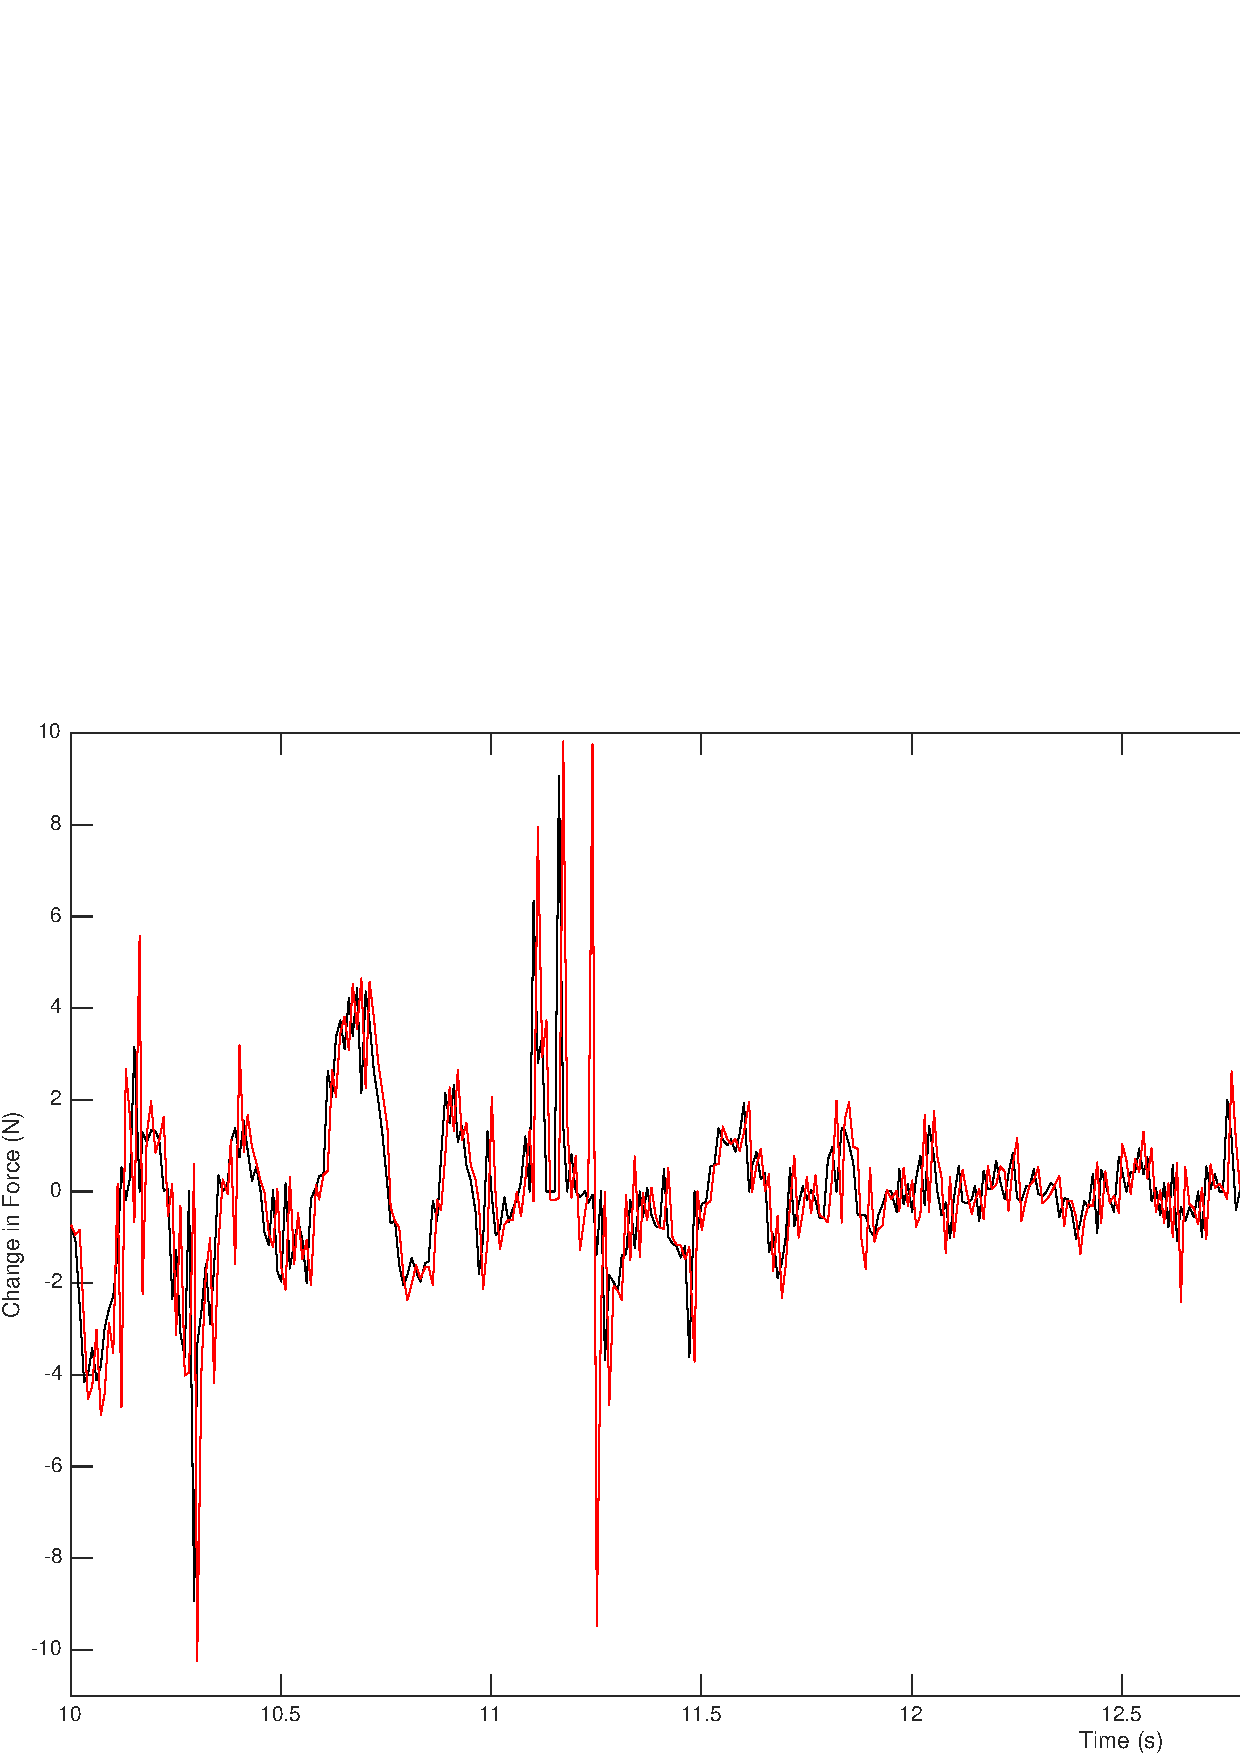
\includegraphics[scale=0.4]{images/force_estimate.pdf}
  \caption{Change of contact force in the vertical direction.  The right foot
    of the iCub is placed on a white foam.}
  \label{force_estimate}
\end{figure}
In order to estimate the contact parameters ($\BK$ and $\BD$), we use locally
weighted projection regression (LWPR) algorithm.  This algorithm gives us a
locally linear model for a non-linear function which suits our application.
The outcome of this algorithm will be $\BK$ and $\BD$ at each time instant
based on the previous values of the contact force and the position and
velocity of the contact point.  Therefore, we can compute the (estimation of
the) contact force in the next instant.  Implementation of this algorithm is
available from \url{https://github. com/azadm/LWR_for_ContactParams.git}.  To
verify this algorithm, TUD performed a few experiments on iCub robot standing
on soft surfaces.  During those experiments, the robot was standing on two
different surfaces (transparent plastic and white foam) while balancing
controller was running on the robot.  The upper body of the robot was
perturbed and data from all sensors were collected in order to calculate the
movements of the contact points and also the contact forces.  By feeding these
values into our LWPR algorithm, we estimated the contact force and compared
with the actual data from F/T sensors.  The results are acceptable and show
the consistency of the LWPR estimation algorithm.  For example,
Fig~\ref{force_estimate} shows the match between actual and estimated change
of the contact force in the vertical direction while the robot's right foot is
on a soft surface (i.e. white foam).
%



\subparagraph*{Extension and enhancement of the iDyn library. (T1.5)}
\label{sec:T15}

As part of this task, IIT has developed a YARP, C++ based  module in charge of implementing a Kalman filter to estimate the floating base position-and-orientation 
(see \url{https://github.com/robotology/codyco-modules/tree/master/src/modules/wholeBodyEstimator}). 
\begin{figure}[t!]
 \centering
 \includegraphics[width=0.4\textwidth]{images/MixCoordSys.png}
 % MixCoordSys.png: 365x315 pixel, 90dpi, 10.30x8.89 cm, bb=0 0 292 252
 \label{fig:coordsys}
 \caption{World reference frame $w$ and local sensor reference frame $\{s\}$. $R(q^{s}_{w})$ denotes the quaternion-based rotation matrix that rotates the world reference frame $w$ into $\{s\}$. }
\end{figure}

In particular,
the goal of this Kalman Filter is to estimate the orientation of a world reference frame $w$ with respect to the sensor reference $\{s\}$ in the quaternion representation (radians), i.e.~$q^{s}_{w}$.  The filter uses only a triad of gyroscopes and accelerometers  along with a simple model of the process representing solely the orientation to be estimated. In this way, the state of the Kalman Filter will be the quaternion-based orientation of the world $w$ in the sensor reference frame $\{s\}$, i.e.
\begin{equation}
  x = q^{s}_{w}
\end{equation}
Where $q = [q_1 \quad q_v]$, $q_1 \in \mathbb{R}$, $q_v \in \mathbb{R}^3$ and $||q|| = 1$. 

The (discrete-time) \emph{process model} of the filter
 is obtained starting off the continuous time equations relating the quaternion orientation with its derivative resulting in the following differential equation:
 \begin{equation}
  \dot{q}^{s}_{w}(t) = \frac{1}{2}\Omega(\omega^{s}(t))q^{s}_{w}(t)
  \label{Eq:diffEq}
 \end{equation}
 Linear approximations of the above dynamics with a fixed-time step assumption leads us to the \emph{process model} of the filter of the form 
 \[x_{k+1} = Ax_k + w_k\]
The \emph{measurement model} of the filter is constituted by the accelerometer only, neglecting its bias and scaling factors or body acceleration. The latter assumption is also done in many commercial IMUs as the one used to compare our results. This leads us to a measurement model of the form
\[z_{k} = h(x_{k+1}) + v_{k}\]
 The measurement model described by the above equation is non-linear in $q$. To fully describe the filter we further need to linearize $h(\cdot)$. 
  Then, we have all the elements necessary to implement an Extended Kalman Filter with linearized measurement equations.
For further details see  \url{https://github.com/robotology-playground/codyco-deliverables/blob/master/D5.3/pdf/D5.3.pdf} Sec. 5.1 \cite{deliverable53}.







%!TEX root = ../../fourthYearReport.tex


\subparagraph*{Resources}
Overall, the use of resources within WP1 was in accordance to the plans. 

\begin{center}
  \begin{tabular}{|C{1.5cm}|C{1.5cm}|C{1.5cm}|C{2cm}|C{2cm}|C{2cm}|C{2cm}|}
    \hline \footnotesize \textbf{WP1 person months}& \footnotesize
    \textbf{IIT}&\footnotesize \textbf{TUD}&\footnotesize \textbf{UPMC}&
    \footnotesize \textbf{UB} &\footnotesize \textbf{JSI} & \footnotesize \textbf{INRIA}\\
    \hline \footnotesize Year 1  & 8.67  & 1.00 & 3.29 & 0.51 & 2.00 & -\\
    \hline \footnotesize Year 2  & 3.00  & 3.00 & 0.47 & 2.29 & -    & - \\
    \hline \footnotesize Year 3  & -     & 1.00 & -    & 2.18 & 2.00 & 2.96 \\
    \hline \footnotesize Year 4  & ?     & 1.00 & 1.31 & ?    & 0.00 & 2.06 \\
   	\hline \footnotesize Partial & ?     & ?    & ?    & ?    & ?    & ?    \\
	\hline
    \hline \footnotesize Overall & 12.00 & 9.00 & 6.00 & 15.00 & 6.00 & 5.00 \\
    \hline
  \end{tabular}
\end{center}

\subparagraph*{Deviations from workplan} 
Overall the project is aligned with the plan.


%!TEX root = ../../secondYearReport.tex
\paragraph{Work package 2 progress}

\subparagraph{Definition and design of experimental protocols (T2.1)}

The aim of the work in this task was to provide a solid multidisciplinary base for future research work within CoDyCo. We made a thorough review and summary of the recent relevant literature on human postural control and whole body motion in contact with environment (Delivery 2.1). The review examines postural control strategies without and with additional support contacts, types of perturbations that are commonly used to study neuromuscular functions involved in postural control and reviews the methods for stability evaluation of bipedal systems. The review is concluded with examination of stability metrics that can be applied for non-planar contacts. We plan to extend the review with methods of determination of inertial parameters of human/robot body and submit it for publication in a robotic journal by the end of 2014.

At JSI, we created an experimental setup to study human postural control and whole body motion in contact with environment. We implemented two state-of-the-art methods for perturbation of balance as shown on Figure \ref{fig:exp_protocol_W2} that will allow us to gain understanding how human brain deals with environment in the sense of supportive contacts. Using the same setup we can also validate all biomechanical findings on robotic systems by simply substituting the human subject with a robot. Besides, work has been undertaken to setup experiments also at UB. New equipment (the Moog Hapticmaster robot) was acquired and configured at both JSI and UB. Hapticmaster robot will be used in experiments with compliant and unpredictable contacts.


\subparagraph{Design of models for human whole body motion in contact (T2.2)}

Work has begun on understanding how to derive simplified models of whole-body balance that will encapsulate the task relevant parameters of posture control with multiple contacts. By emulating situations when balance of an individual is challenged, we examined functional role of supportive hand contact at different locations where balance of an individual was perturbed by translational perturbations of the support surface. The experimental methods rested upon our work in Task 2.1 and are depicted on the left side of Figure \ref{fig:exp_paper_W2}.


We found that an additional supportive hand contact significantly reduced the maximal displacement of the subject's centre of pressure (CoP) regardless of the position of the handle and the type of the perturbation. On the other hand, the position of the handle had no effects on the maximal CoP displacement (top right diagram on Figure \ref{fig:exp_paper_W2}) which is against the previous belief that the quality of postural control depend on the location of the hand contact \cite{Sarraf2014} and supports the idea that maintaining postural stability is the task of the highest priority and that the central nervous system does whatever necessary to keep the body balanced \cite{Winter1995}. Specifically, subjects always generated the required hand force, no matter where the location of the handle was, to keep the body balanced to the same extent. To get a better understanding of the functional role of supportive hand contacts, we examined the handle forces exerted by the subjects during the perturbation. In contrast with the effects on CoP, we found significant effects of perturbation direction, perturbation intensity and handle position on the maximal force in the handle (bottom right diagram on Figure \ref{fig:exp_paper_W2}). A manuscript with the results of the work in T2.2 was submitted for publication in Gait \& Posture journal in December 2013 and is under review \cite{Babic2014}.

To properly model all these findings we developed a reduced dimensional (6-link, planar) model of a humanoid to be used as an inverse dynamics model for computing joint torques from human experimental data. The detailed analyses based on this model are under way at JSI and UB.

A major challenge of this task is understanding how to determine and measure stability when a human or humanoid robot is in a multi contact situation. The state-of-the-art in postural stability uses traditional metrics such as centre of pressure or zero moment point. However these planar metrics do not apply when there are multiple non-planar contacts. In addition to reviewing the current literature (Task 2.1), we have begun development of new methods for measuring stability margins when a human or humanoid robot has multiple non-planar contacts.

\subparagraph{Human contact choice and learning through physical interaction (T2.4)}

In order to understand how humans make contact choice decisions (e.g. whether or not to initiate a hand contact, and where to place the hand), we need an estimation of joint torques as well as a metric of stability in various multi-contact situations. Thus the work we have begun in Task 2.2 in terms of both simplified models of postural control and metrics of stability, also apply for Task 2.4.

To understand the factors involved in human choice of contact utilization, we performed a series of experiments where the subjects were standing still with arms hanging freely at the sides. The parallel platform induced a randomly timed series of perturbations of different accelerations, velocities and displacements. The aim of the experiments was to investigate what profile of support perturbation forces the human to make a supportive hand contact with environment and how human chooses the location of the hand contact with regard to the direction of the perturbation. Interestingly, we found that the subjects reacted to every perturbation no matter how small or slow the perturbation was or what was the initial acceleration of the perturbation. The reactions were manifested as muscle twitches of shoulder or as unspecific arm motions that were unrelated to the proximity of possible support objects. The reactions occurred also at the smallest perturbations when no actual correction of balance was needed. Our experiments showed that these reactions are essentially protective reactions rather than reactions that have counterbalancing effects \cite{McIlroy1995, Corbeil2013}.

These reactions mask the real factors involved in human choice of contact utilization. We therefore altered the perturbation methods for our further experiments and designed continuous random perturbations in a frequency band that corresponds with typical human motion during postural control \cite{Nawayseh2006}. By doing so we excluded the effect of surprise that evoked the reflex reactions of humans. This will hopefully allow us to uncover the factors involved in human choice of contact utilization.

%!TEX root = ../../fourthYearReport.tex
\subparagraph*{Resources}
Overall, the use of resources within WP2 was in accordance to the plans. 

\begin{center}
\begin{tabular}{|C{1.5cm}|C{1.5cm}|C{1.5cm}|C{2cm}|C{2cm}|C{2cm}|C{2cm}|}
\hline
\footnotesize \textbf{WP2 person months}& \footnotesize \textbf{IIT}&\footnotesize \textbf{TUD}&\footnotesize \textbf{UPMC}& \footnotesize \textbf{UB} &\footnotesize \textbf{JSI} & \footnotesize \textbf{INRIA} \\ \hline
\footnotesize Year 1  &  -     & -    & 0.28 & 2.64  & 18.80  & -     \\  \hline
\footnotesize Year 2  &  -     & 3.00 & 0.48 & 7.67  & 21.85  & -     \\  \hline
\footnotesize Year 3  &  -     & 1.00 & 1.20 & 13.88 & 21.69  & 0.52  \\  \hline
\footnotesize Year 4  &  -     & 3.00 & 0.75 & 21.50 & 20.00  & 1.00  \\  \hline 
\footnotesize Partial & ?      & ?    & ?    & ?     & ?      & ?     \\
\hline \hline
\footnotesize Overall & -      & 4.00 & 1.00 & 45.00  & 55.00 & 1.00  \\  \hline
\end{tabular}
\end{center}

\subparagraph*{Deviations from workplan} 
No significant deviations.


%!TEX root = ../../secondYearReport.tex


 
\paragraph{Work package 3 progress}

The progress for each task are described hereafter.

\subparagraph{Reproducing existing control results in a simple case (T3.1)}
During year one, UPMC has achieved task T3.1 by creating a stand-alone C++ library encapsulating the whole-body controller developed in \cite{salini2012} so that it can be used by all partners in simulation or on (any) real humanoid robot. This version of the controller has been tested in rigid multi-contact scenarios in simulation (see Fig.~\ref{fig:xde}) and is currently adapted for tests on the iCub robot.


\subparagraph{Formulating the control problem (T3.2)}

The work performed during year one by UPMC to achieve T3.2 has led to the definition of what a task can be considered to be in the context of the reactive formulation of a multi-task whole body control problem. Among the different characteristics of a task (physical frame, task variable, forward model, desired target trajectory, local controller, priority), the notion of task priority has been largely modified with respect to the classical lexicographic task ordering met in the robotics literature and which is particularly appropriate for cascade resolution approaches such as the one recently proposed in \cite{escande2012}. A partial order has been defined such that task priorities can be described for any pair of task $i$ and $j$. This leads to a richer formulation which includes the original one but is also particularly appropriate for describing task insertion and removal processes as well as priority switching between tasks. Further more, this new prioritization paradigm provides a unique way of defining strict and soft hierarchies between tasks. Associated to this work, the notion  of generalized task projector has been introduced. Each task is associated to a projector which is built based on the tasks priorities. The interest of this projector is that it filters the joint space motion associated to a task so that all priorities are respected, being them soft or strict. Details regarding this work are provided in \cite{liu2013}.

Within this task also IIT contributed with the definition of a software abstraction layer, named wholeBodyInterface (\url{http://wiki.icub.org/codyco/dox/html/namespacewbi.html}). This software library defines the interface to access and control the robot  whole-body. Therefore the wholeBodyLibrary structures the control problem and their definition. Currently the library has been been implemented for both the iCub and the Gazebo iCub simulator.  

\subparagraph{Solving the local control problem (T3.3)}

Associated to the new task formulation proposed in T3.2, the control problem has been formulated by UPMC as an LQP which can be solved by any convex optimization solver dealing with linear constraints. Despite the task hierarchy, the introduction of a generalized task projector per task allows to solve only one LQP. This can be done by introducing as many virtual joint space variables as the number of tasks and using the generalized projector of each task in the expression of the constraints. The resulting problem can be solved by standard convex optimization tools and the cost of introducing virtual joint space variables is compensated for by the fact that only one optimization problem has to be solved. Details regarding this work are provided in \cite{liu2013}.

In the meantime, TUD has proposed to explore optimization methods for solving local control problems that do not require the explicit inversion of any model of the system.  During year one, TUD investigated Bayesian optimization methods that were applied to bipedal locomotion tasks.  One of the key challenges in robotic bipedal locomotion is finding gait parameters that optimize a desired performance criterion, such as speed, robustness or energy efficiency. Typically, gait optimization requires extensive robot experiments and specific expert knowledge. During year one, TUD demonstrated that  data-driven machine learning methods based on Bayesian optimization can be used to automate and speed up the process of gait optimization. These Bayesian optimization methods were used to efficiently find gait parameters that optimize the desired performance metric on a real bipedal walker \cite{calandra2014} and \cite{calandra2014b}.
    

\subparagraph{Bootstrapping and validating the control approach in rigid world and compliant cases (T3.4)}

During year one, UPMC has explored the contribution of MPC approaches to handle the postural balancing problem under varying contact conditions. The hybrid nature of the problem, where varying contact conditions can be accommodated either by adapting the internal forces distribution given a set of contact or by modifying the set of contacts itself, requires control approaches where the desired task trajectories performed through the local, reactive, whole-body controller have to be optimally planned ahead of time in order to provide robust behaviors. The contributions in this domain are mostly related to the work of A. Ibanez \cite{ibanez2013}, \cite{ibanez2014-icra} and \cite{ibanez2014-ark}. The originality of theses contributions lies in:
\begin{itemize}
	\item an augmented ZMP model including external forces exerted directly on indirectly on the center of mass;
	\item a distributed optimization approach that provides a way of generating reference trajectories for the center of mass representing a good compromise given some antagonistic balance and task;
	\item a non scripted foot step placement optimization.
\end{itemize}

UPMC also partially contributed with an experimental study about human behavior during physical contact with the robot. The protocol was registered and obtained the approval of the ethics committee CERES (Conseil d’\'evaluation \'ethique pour les recherches en sant\'e), from University Paris-Decartes. \footnote{Ivaldi et al., "Engagement during human-humanoid interaction", IRB N. 20135200001072.}
The purpose of the experiments is to collect a database of behaviors of experts and naive people interacting physically with the iCub to accomplish a cooperative task. The collected data also include locations of contacts (retrieved through the tactile skin), applied force, robot mouvements: they will be used to study adaptation to human intention during human-robot physical contacts.
    
In the meantime, TUD investigated the interchange of forces during cooperative tasks between humans and robots \cite{berger2013}. Three example scenarios are illustrated in Figure \ref{fig:interaction_tasks}. In such tasks, typically an exchange of forces takes place whenever the interacting agents make contact. Sometimes, forces are even exchanged through an object that is manipulated by both agents, e.g., through a box that is lifted. For a successful execution of such joint physical activities, a robot needs to accommodate for the external forces exerted by a human. To this end, we developed a machine learning approach for identifying external influences and guidance information from humans. During behavior execution by a robot, predictions from a statistical sensor model are continuously compared with stability parameters derived from current sensor readings. Differences between predicted and measured values exceeding the variance of the statistical model are interpreted as perturbations caused by a human and are used to adapt the robot's behavior.
    
\subparagraph{Deviations from workplan}  

The PM expenses for WP3 after one year of project are globally conform to the planned one. The observed deviations are related to the fact that tasks 3.3 and 3.4 spans the overall duration of the project and the contribution of some of the partners are expected in the 2nd, 3rd and 4th year.

%\emph{\color{red}[For work package 3 (UPMC) provide the following information:]}
%\begin{itemize}
%\item[-] \emph{\color{red}[A summary of progress towards objectives and details for each task;]}
%\item[-] \emph{\color{red}[Highlight clearly significant results;]}
%\item[-] \emph{\color{red}[If applicable, explain the reasons for deviations from Annex I and their impact on other tasks as well as on available resources and planning;]}
%\item[-] \emph{\color{red}[If applicable, explain the reasons for failing to achieve critical objectives and/or not being on schedule and explain the impact on other tasks as well as on available resources and planning (the explanations should be consistent with the declaration by the project coordinator) ;]}
%\item[-] \emph{\color{red}[a statement on the use of resources, in particular highlighting and explaining deviations between actual and planned  person-months per work package and per beneficiary in Annex 1 (Description of Work);]}
%\item[-] \emph{\color{red}[If applicable, propose corrective actions.]}
%\end{itemize}





%!TEX root = ../../fourthYearReport.tex

\subparagraph{Resources}

\begin{center}
\begin{tabular}{|C{1.5cm}|C{1.5cm}|C{1.5cm}|C{2cm}|C{2cm}|C{2cm}|C{2cm}|}
\hline
\footnotesize \textbf{WP3 person months} & \footnotesize \textbf{IIT}&\footnotesize \textbf{TUD}&\footnotesize \textbf{UPMC}& \footnotesize \textbf{UB} &\footnotesize \textbf{JSI} &\footnotesize \textbf{INRIA} \\ \hline
\footnotesize Year 1  &  9.90 & 4.60  & 15.15 & -    & -    &  -   \\  \hline
\footnotesize Year 2  &  -    & 10.5  & 14.67 & 1.85 & 1.00 & 4.14  \\  \hline
\footnotesize Year 3  &  -    & 9.65  & 8.79  & 1.63 & 2.00 & 4.03 \\  \hline
\footnotesize Year 4  & ?     & 3.6   & 8.51  & ?    & 1.00 & 1.98    \\   	\hline
\footnotesize Overall & ?     & 28.35 & 47.12 & ?    & 4.00 & 10.15    \\
\hline \hline
\footnotesize Planned &  9.00 & 24.00 & 43.5 & 10.00 & 4.00 & 10.50 \\ \hline
\end{tabular}
\end{center}

%In order to best use the whole-body controllers developed within the framework of WP3, TUD hired a student for setting up the iCub hardware and simulation environment.

\subparagraph*{Deviations from workplan}

No major deviation from the workplan was observed.



%!TEX root = ../../thirdYearReport.tex


\paragraph{Work package 4 progress}

\subparagraph*{Improved Models from Real-Time Regression with Latent Contact Type Inference (T4.1)}

Within T4.1 IIT developed in the first and the second year of the 
project a theoretical framework for estimating whole-body
dynamics from distributed multimodal sensors \cite{nori2015}. The sensors considered
include joint encoders, gyroscopes, accelerometers and force/torque sensors. In the third year of the project, IIT investigated the integration of this estimation techniques with the classical identification techniques for inertial parameters \cite{traversaro2015parametersEM}. For the fourth year the improvement of the reliability of the sensors was considered. More specifically the six axis force/torque sensors where discovered to have a change in behaviour after they are mounted on the robot. To tackle this an in-situ calibration procedure was developed.

The procedure used to calibrate the sensors in-situ takes advantage of the knowledge of the model of the robot to generate the expected wrenches of the sensors during some arbitrary motions. The wrenches used as reference are estimated through the model and kinematic measurements. It then uses this information to train and validate new calibration matrices, taking into account the calibration matrix obtained with a classical Workbench calibration.  This procedure was validated  on the F/T sensors mounted on the iCub humanoid robot legs and published in Humanoids 2016 \cite{Andrade}.


\begin{figure}
        \centering
        \includegraphics[width=.45\textwidth]{images/all1valid2.png}
        \caption{3D force comparison among the calibration matrices trained on each dataset against the model estimated forces on the fastExtBal1 dataset. }
        \label{fig:all1valid}
\end{figure}



% bibliography 
%@inproceedings{nori2015,
%  title={Simultaneous state and dynamics estimation in articulated structures},
%  author={Nori, Francesco and Kuppuswamy, Naveen and Traversaro, Silvio},
%  booktitle={Intelligent Robots and Systems (IROS), 2015 IEEE/RSJ International Conference on},
%  pages={3380--3386},
%  year={2015},
%  organization={IEEE}
%}
%
%@article{traversaro2015parametersEM,
%  title={Dynamic parameters identification in articulated rigid bodies with redundant heterogeneous sensors},
%  author={Traversaro, Silvio and Venture, Gentiane and Nori, Francesco},
%  booktitle={Submitted},
%}
%
%@INPROCEEDINGS{Andrade,
%author={F. J. Andrade Chavez and S. Traversaro and D. Pucci and F. Nori},
%booktitle={2016 IEEE-RAS 16th International Conference on Humanoid Robots (Humanoids)},
%title={Model based in situ calibration of six axis force torque sensors},
%year={2016},
%pages={422-427},
%doi={10.1109/HUMANOIDS.2016.7803310},
%month={Nov},}


\subparagraph*{Inferring the Operational Space and Appropriate Controls with Multiple Contacts (T4.2) (TUD: 6PM)}%(TUD 4PM, ??PARTNERS)}

%TUD

%Elmar 
During year two, TUD and JSI investigated the effect of supportive contacts on 
postural control. First results were presented during the second year review 
meeting (Task T2.4 on Human contact choice and learning through physical 
interaction). During year three, we collected a large dataset of more than 
$9.000$ reaching movements in $20$ subjects. To analyze the data TUD developed a 
probabilistic model which extends classical statistical tests (ANOVA test of 
contact locations and target locations, movement onsets, etc.). The 
probabilistic model allows for detailed investigations of movement kinematics in 
a spaciotemporal domain and extends classical techniques that rely on scalar 
descriptors of the complex motion patterns. In whole body adaptation 
experiments, shown in Figure \ref{fig:subFigContactLocationsAllSubjects}, TUD 
and JSI found strong correlations between both arms and the trunk. These 
correlations were used to predict the reaching motion from early phase 
observations of the supportive contact motion. The results suggest that postural 
control predicts and precedes goal-directed movements, which has the potential 
to impact pre-tests of central nervous system disorders like dementia, 
Alzheimer's or Parkinson's disease that are less prone to factors like stress, 
sleep deprivation and age compared to the classical cognitive tests. A pre-print 
of a paper that was submitted for review to Scientific Reports is given in 
Deliverable D2.2.

\begin{figure}%[t]
\centering
\includegraphics[width=\textwidth]{images/Figure-1(rueckert)}
%\label{fig:subfig2}
 \caption[Human reaching experiment with target dependent contacts and synchronized arm motions.]{\textbf{Experiment, target dependent contacts and synchronized arm motions.} \textbf{A)} Experimental setting. 
 \textbf{B)}  The top row shows contact locations for a single representative subject 
 and the bottom row shows the mean and the confidence bound over all $20$ participants. 
 The first $80$ trials and the last $80$ trials are unperturbed sessions. 
 Catch trials were initiated during trials $240$ to $400$ and are denoted by the black lines in \textbf{B}.
 \textbf{C)} Illustration of the movement onsets of the wrists for the first five trials. 
 \textbf{D)} Movement onsets for the first six trials transitioning to the perturbed session. 
}
\label{fig:subFigContactLocationsAllSubjects}
\end{figure}

In ongoing work, TUD and JSI investigate how such probabilistic models can predict when 
and how to make supportive contacts in robot reaching tasks. Our goal is to 
reproduce the correlated reaching and supportive contact motions in the iCub robot. 
In addition to the target dependent contact locations, a module that predicts 
when to initiate a supportive contact will be developed. This model will make 
use of the estimated center of pressure using the two force/torque sensors in the 
ankles. 

\begin{figure}
\centering
\includegraphics[width=\textwidth]{images/KukaLearnedModelObstacles}
%\label{fig:subfig2}
 \caption[Planning in spkining neural networks with multiple constraints on a Kuka robot.]{\textbf{Planning with multiple constraints on a real robot.} {\bf A)} Generated 
spike train (top: context neurons, bottom: state neurons) after contrastive 
divergence learning of the transition model. {\bf B)} Two sampled movement plans 
solving the obstacle avoidance task. {\bf C)} Snapshots of the executed movement 
on the real robot.
}
\label{fig:exp_kukaRueckert}
\end{figure}

In another approach, TUD investigated computational models of operational space 
control in rodents using spiking neural networks. While this study is more of a 
fundamental type and does not directly provide concrete algorithms for humanoid 
robot control, it has interesting potentials for the challenging tasks in 
CoDyCo. Concretely, in spiking neural networks arbitrary-shaped obstacles can be 
modeled, non-linearities in the transition model due to contacts can be learned 
and movement plans can computed much faster then real-time through exploiting 
local-only dependencies. These advantages were evaluated in target-reaching task 
in a Kuka robot arm. For that TUD developed learning algorithms grounded in the 
theory of probabilistic inference to train the recurrent spiking neural network 
from human demonstrations. The training data was collected in kinesthetic 
teaching. After the training, the network model was used to plan goal-directed 
task space trajectories that avoid obstacles in the three-dimensional space. Two 
example movements and the corresponding neural activity are illustrated in 
Figure \ref{fig:exp_kukaRueckert}. For details on the approach we refer to 
Deliverable D4.1. A manuscript on this work was accepted for publication in 
Scientific Reports~\cite{Rueckert_SR_2016} (impact factor 5.578 in 2014). 

In a student's master thesis, TUD extended the model to jointly model 
configuration and task spaces. This extension is based on factorized population 
codes and allows for applications to high-dimensional robot systems. In ongoing 
work, TUD will test the learning algorithms of the spiking network in the iCub 
robot.    


\subparagraph*{Learning the Prioritization of Tasks (T4.4) (TUD: 6PM, UPMC: 0.74)}%(TUD 3.2PM, INRIA 2PM)}

During the third year, TUD continued its research on learning controllers for 
physical interaction. We presented a novel approach at an international robotics 
conference~\cite{paraschos2015model}. The approach learns and generates 
movements for physical interaction that are trained with imitation learning from 
a small set of demonstrated trajectories. Learning such a model is a non-trivial 
task and therefore we introduced the \textit{model-free} Probabilistic Movement 
Primitives (ProMPs). Here, we learn jointly the movement and the necessary 
actions from a few demonstrations. We derived a variable stiffness controller 
analytically and we extended the ProMPs to include force and torque signals, 
necessary for physical interaction in the CoDyCo scenarios. 

Based on these results we also focused on developing a novel approach for task 
prioritization during year three. Our approach follows the concept of ``soft'' 
priorities, where a task which is lower in the task-hierarchy can controllably 
interfere with a higher-priority task. This concept is applicable to a wide-set 
of problems including balancing and reaching in humanoids with physical contacts 
with the environment. In our approach we dynamically change the priority of each 
task in time and, thus, adapt the behavior of the robot dynamically.  The 
approach utilizes imitation learning to obtain the variance of each task 
movement which is then used as the relative priority of the task. An important 
contribution of our approach shows how we can utilize probabilistic methods to 
analytically derive the tasks priorities from the imitation learning. We relate 
our approach to other state-of-the-art movement prioritization 
approaches~\cite{Peters_AR_2008, lober2015variance} and we show how these 
approaches can be derived under our framework. We provide an alternative point 
of view on movement prioritization that is derived from first-order principles. 
We demonstrated that our approach achieves improved performance and that is 
numerically stable, avoiding singularities. A paper on this approach was 
submitted to a robotics conference.

UPMC developed whole-body controllers allow multiple concurrent tasks to be 
executed on redundant robots, and such combinations often engender unforeseeable 
incompatibilities between the tasks due to conflicting task objectives and the 
robot's constraints. The result is typically a failure of one or more tasks to 
be properly carried out. In \cite{lober-HUMANOIDS2014}, UPMC introduced a measure of task 
compatibility, or compatibility cost. By optimizing parametric task 
representations, UPMC was able to minimize said cost and render the tasks 
compatible, albeit slowly. In \cite{lober2015variance}, UPMC looked at how task 
priorities could be automatically modulated by the variance associated with each 
task. This provided a reactive way to handle many common incompatibility 
scenarios. Currently, lately UPMC has been working on more computationally 
efficient task compatibility optimization schemes which combine the previous two 
works.   

  INRIA, in collaboration with TUD, has been working on the problem of automatically optimizing the soft task priorities for multi-task controllers.
      The goal of this work is to facilitate the automatic tuning of the task weights and task transitions when multiple elementary tasks are used to realize a more complex "global" task or movement.  When the number of tasks increases, for example in whole-body control of humanoid robots, it is generally difficult to define suitable task activations: the task weights/priorities and their transitions are manually tuned by expert users or defined before-hand. In \cite{Modugno2016}, INRIA proposed a framework to automatically optimise the soft task priorities by means of a stochastic optimization algorithm. In the framework, the temporal profiles of the task weights, approximated by a mixture of Gaussian, can be learned by optimizing a given fitness function used to evaluate the performance of the candidate task priorities.  Optimization was done by the state-of-the-art CMA-ES algorithm. The method has been evaluated on the redundant manipulator Jaco and a simulated KUKA LWR, showing that it improves the fitness of the gloabl movement and the smoothness of the joint trajectories (see Figure  \ref{fig:valerio:framework}). The work has been also presented in \cite{Modugno2015hfr}.
Currently, INRIA is working towards two main improvements on this framework: 1) to scale-up the framework to the iCub, to study its performance in handling several DOF and several tasks; 2) to include the constraints evaluation in the optimization process, such that the optimization process always generates solutions that cannot violate constraints; this is done by guiding the exploration with both the fitness and the constraints violations functions: preliminary results indicate that a (1+1)-CMA-ES seems to be the best candidate algorithm to address this issue (see Figure  \ref{fig:valerio:constraints}). A paper is in preparation.

\begin{figure*}[h!]
    \centering
    \begin{subfigure}[t]{0.9\textwidth}
        \centering
      \includegraphics[height=3cm]{images/v_alphas_hand}
	\includegraphics[height=3cm]{images/v_alpha_combine}
	\includegraphics[height=3cm]{images/v_fitness_comp_3task_kinova1}
    \caption{Manually tuned vs optimized task weights (solid line: fixed init, dashed line: random init). The fitness for the optimizes weights is smaller (better). More in \cite{Modugno2016}.}
        \label{fig:valerio:framework}
    \end{subfigure}%
    
    \begin{subfigure}[t]{0.9\textwidth}
        \centering
        \includegraphics[height=4.5cm]{images/v_to_steady.png}
        \includegraphics[height=4.5cm]{images/v_viol.png}
        \caption{Comparison of three variants of constrained CMA-ES on benchmarks. (1+1)-CMA-ES never violates the constraints, despite requiring more time to converge to the optimal solution.}
        \label{fig:valerio:constraints}
    \end{subfigure}
    \caption{}
\end{figure*}


%!TEX root = ../../secondYearReport.tex

\subparagraph{Resources}

\begin{center}
\begin{tabular}{|C{1.5cm}|C{1.5cm}|C{1.5cm}|C{2cm}|C{2cm}|C{2cm}|C{2cm}|}
\hline
\footnotesize \textbf{WP4 person months}& \footnotesize \textbf{IIT}&\footnotesize \textbf{TUD}&\footnotesize \textbf{UPMC}& \footnotesize \textbf{UB} &\footnotesize \textbf{JSI} &\footnotesize \textbf{INRIA}\\ \hline
\footnotesize Year 1 &  0.00 & 8.00 & 2.22 & 0.00 & 0.00 & -     \\  \hline
\footnotesize Year 2 &  6.04 & 21.70 & 1.69 & 2.15 & 3.00 & 2.01     \\  \hline
\footnotesize Partial &  6.04 & 29.70 & 3.91 & 2.15 & 3.00 & 2.01 \\ \hline \hline
\footnotesize Overall &  30.00 & 38.00 & 9.00 & 12.00 & 10.00 & 9.00 \\ \hline
\end{tabular}
\end{center}

\subparagraph{Deviations from workplan} 
Six person months of UPMC planned for Serena Ivaldi were transfered to TUD. No significant deviations. 


%!TEX root = ../../thirdYearReport.tex

\paragraph{Work package 5 progress}

Summary.

\subparagraph{Result 1}

Some result.

\subparagraph{Result 2}

Some result.
%!TEX root = ../../secondYearReport.tex

\subparagraph{Resources}

Resources were used with small difference with respect to what planned. In particular IIT invested only 2 PM with respect to 12PM planned. The motivation resides in the fact that WP5 took advantage of the significant effort done in WP1 (software) and WP3 (control) and in a sense resources initially planned on T5.1 eventually have been committed to T1.1, T1.2, T1.3, T3.1 and T3.2.

\begin{center}
\begin{tabular}{|C{1.5cm}|C{1.5cm}|C{1.5cm}|C{2cm}|C{2cm}|C{2cm}|C{2cm}|}
\hline
\footnotesize \textbf{WP5 person months}& \footnotesize \textbf{IIT}&\footnotesize \textbf{TUD}&\footnotesize \textbf{UPMC}& \footnotesize \textbf{UB} &\footnotesize \textbf{JSI} & \footnotesize \textbf{INRIA} \\ \hline
\footnotesize Year 1 &  2.00 & 0.00 & 0.31 & 0.00 & 0.00 & 0.00     \\  \hline
\footnotesize Year 2 &  12.00 & 0.00 & 0.05 & 0.00 & 0.00 & 0.00     \\  \hline
\footnotesize Partial &  14.00 & 0.00 & 0.36 & 0.00 & 0.00 & 1.50 \\ \hline \hline
\footnotesize Overall &  48.00 & 5.00 & 2.50 & 0.00 & 0.00 & 1.50 \\ \hline
\end{tabular}
\end{center}

\subparagraph{Deviations from workplan} 
The original work plan was leaving quite a flexible set of possibilities for both the postural task (e.g. sitting on a chair or balancing on the feet) and the goal oriented action (e.g. opening a drawer while standing or manipulating object while sitting). In the final validation scenario it was chosen to consider a interactive scenario, with the torque controlled iCub standing on his feet while trying to grasp an object moved by the experimenter. As soon as the object exceeds the robot workspace, the iCub takes a forward step in order to increase his workspace. 

UPMC covered the activities within WP5 with own resources for a total of 0.45 PM. In particular Ryan Lober (PhD student, French PhD research grant) and Darwin Lau (Postdoctoral scholar) participated to the deployment of the whole-body interface developed in WP1 on the iCub robots present at UPMC. TUD covered the activities within WP5 with own resources for a total of 0.5 PM. In particular Serena Ivaldi contributed to the preparation of the second year validation scenario.


%!TEX root = ../../thirdYearReport.tex


\paragraph{Work package 6 progress}

Activities within work package 6 achieved the expected results both in terms of administrative activities and management activities. As a major achievement, the management successfully concluded a third amendment to include INRIA as a partner. The inclusion was motivated by the the new position of Dr. Serena Ivaldi, currently researcher at INRIA, Nancy. 

\subparagraph{Administrative coordination (T6.1)}
Administration was successfully coordinated by IIT, with significant contribution from Chiara Andreoli (iCub Facility), Francesca Boscolo (project offices) and Maria Carmela Fierro (Robotics, Brain and Cognitive Science Department). The major activity concerned the amendment that the CoDyCo consortium asked the main reason being the fact that Serena Ivaldi, initially hired by UPMC and successively moved to TUD, was recently hired by INRIA as researcher. Part of the administrative coordination activities were also conducted during the mid-year meeting: November 20th-21st, 2014, Ljubljana.  Details on the meetings can be found in the CoDyCo website (\url{http://www.codyco.eu}).

\subparagraph{Software repository implementation (T6.2)}

The github software repository was several times restructured \url{https://github.com/robotology/codyco} and the contribution from the different developers can be directly checked in the website. 
%!TEX root = ../../fourthYearReport.tex


\subparagraph*{Resources}

Resources were used as follows.

\begin{center}
\begin{tabular}{|C{1.5cm}|C{1.5cm}|C{1.5cm}|C{2cm}|C{2cm}|C{2cm}|C{2cm}|}
\hline
\footnotesize \textbf{WP6 person months}& \footnotesize \textbf{IIT}&\footnotesize \textbf{TUD}&\footnotesize \textbf{UPMC}& \footnotesize \textbf{UB} &\footnotesize \textbf{JSI} & \footnotesize \textbf{INRIA} \\ \hline
\footnotesize Year 1 &  1.46 & - & 0.25 & - & - & -    \\  \hline
\footnotesize Year 2 &  1.50 & - & 0.31 & - & - & -     \\  \hline
\footnotesize Year 3 &  1.51 & 1.00 & 0.19 & - & 0.44 & - \\ \hline
\footnotesize Year 4  & ?     & ?    & ?    & ?    & 0.54    & ?    \\   	\hline
\footnotesize Partial & ?     & ?    & ?    & ?    & ?    & ?    \\
\hline \hline
\footnotesize Overall &  5.00 & 1.00 & 1.00 & 0.60 & 1.00 & - \\ \hline
\end{tabular}
\end{center}

\subparagraph*{Deviations from workplan} 
JSI budgeted approximatively 29PMs for the year 4. They are higher than planned but with the same reason as already communicated with PO in previous years 


%!TEX root = ../../fourthYearReport.tex


\paragraph{Work package 7 progress}

Dissemination and exploitation activities included the participation to international events addressed to both commercial and academic institutions. 

\subparagraph{Dissemination activities towards academia, industry, and other users (T7.1)}

The explicit goal of T7.1 for the fourth year was to $\dots$

We achieved the following results $\dots$

\subparagraph{Exploitation plan (T7.2)}

The explicit goal of T7.2 for the fourth year was to $\dots$

We achieved the following results $\dots$

\subparagraph{Management of IPR (T7.3)}

The explicit goal of T7.3 for the fourth year was to $\dots$

We achieved the following results $\dots$

\subparagraph{Dissemination of a database of human motion with contacts (T7.4)}

The explicit goal of T7.4 for the fourth year was to $\dots$

We achieved the following results $\dots$

%!TEX root = ../../fourthYearReport.tex


\subparagraph*{Resources}

Resources were used as follows.

\begin{center}
\begin{tabular}{|C{1.5cm}|C{1.5cm}|C{1.5cm}|C{2cm}|C{2cm}|C{2cm}|C{2cm}|}
\hline
\footnotesize \textbf{WP7 person months}& \footnotesize \textbf{IIT}&\footnotesize \textbf{TUD}&\footnotesize \textbf{UPMC}& \footnotesize \textbf{UB} &\footnotesize \textbf{JSI} & \footnotesize \textbf{INRIA} \\ \hline
\footnotesize Year 1 &  1.00 & -    & 0.40 & -    & -    & - \\  \hline
\footnotesize Year 2 &  -    & -    & 0.13 & -    & -    & 0.91 \\  \hline
\footnotesize Year 3 &  1.00 & - & 0.11 & - & - & - \\ \hline
\footnotesize Year 4  & ?     & ?    & ?    & ?    & 1.00    & ?    \\   	\hline
\footnotesize Partial & ?     & ?    & ?    & ?    & ?    & ?    \\
\hline \hline
\footnotesize Overall & 3.00 & 1.00 & 1.00 & 1.00 & 1.00 & 1.00 \\ \hline
\end{tabular}
\end{center}

\subparagraph*{Deviations from workplan} 
No significant deviations. 


\subsection{Deliverables and milestones tables}

\subsubsection{Deliverables (excluding the periodic and final reports)}

\begin{figure*}[ht!]
\centering
\includegraphics[width=0.6\textwidth]{./images/deliverables.pdf}
\end{figure*}

\subsubsection{Milestones}

\begin{figure*}[ht!]
\centering
\includegraphics[width=\textwidth]{./images/milestones.pdf}
\end{figure*}

\newpage

\bibliographystyle{IEEEtran}
% \bibliography{IEEEabrv,yearReport_WP3,all-ias-publications}
\bibliography{secondYearReport_WP4,secondYearReport_WP3,secondYearReport_WP2,secondYearReport_WP1}

\end{document}

%%% Local Variables:
%%% mode: latex
%%% TeX-master: t
%%% save-place: t
%%% End:
